% textidote: ignore begin
\appendix
% textidote: ignore end
\chapter{Appendix}

The appendix includes the original task description and selected notes from the meetings with supervisors.

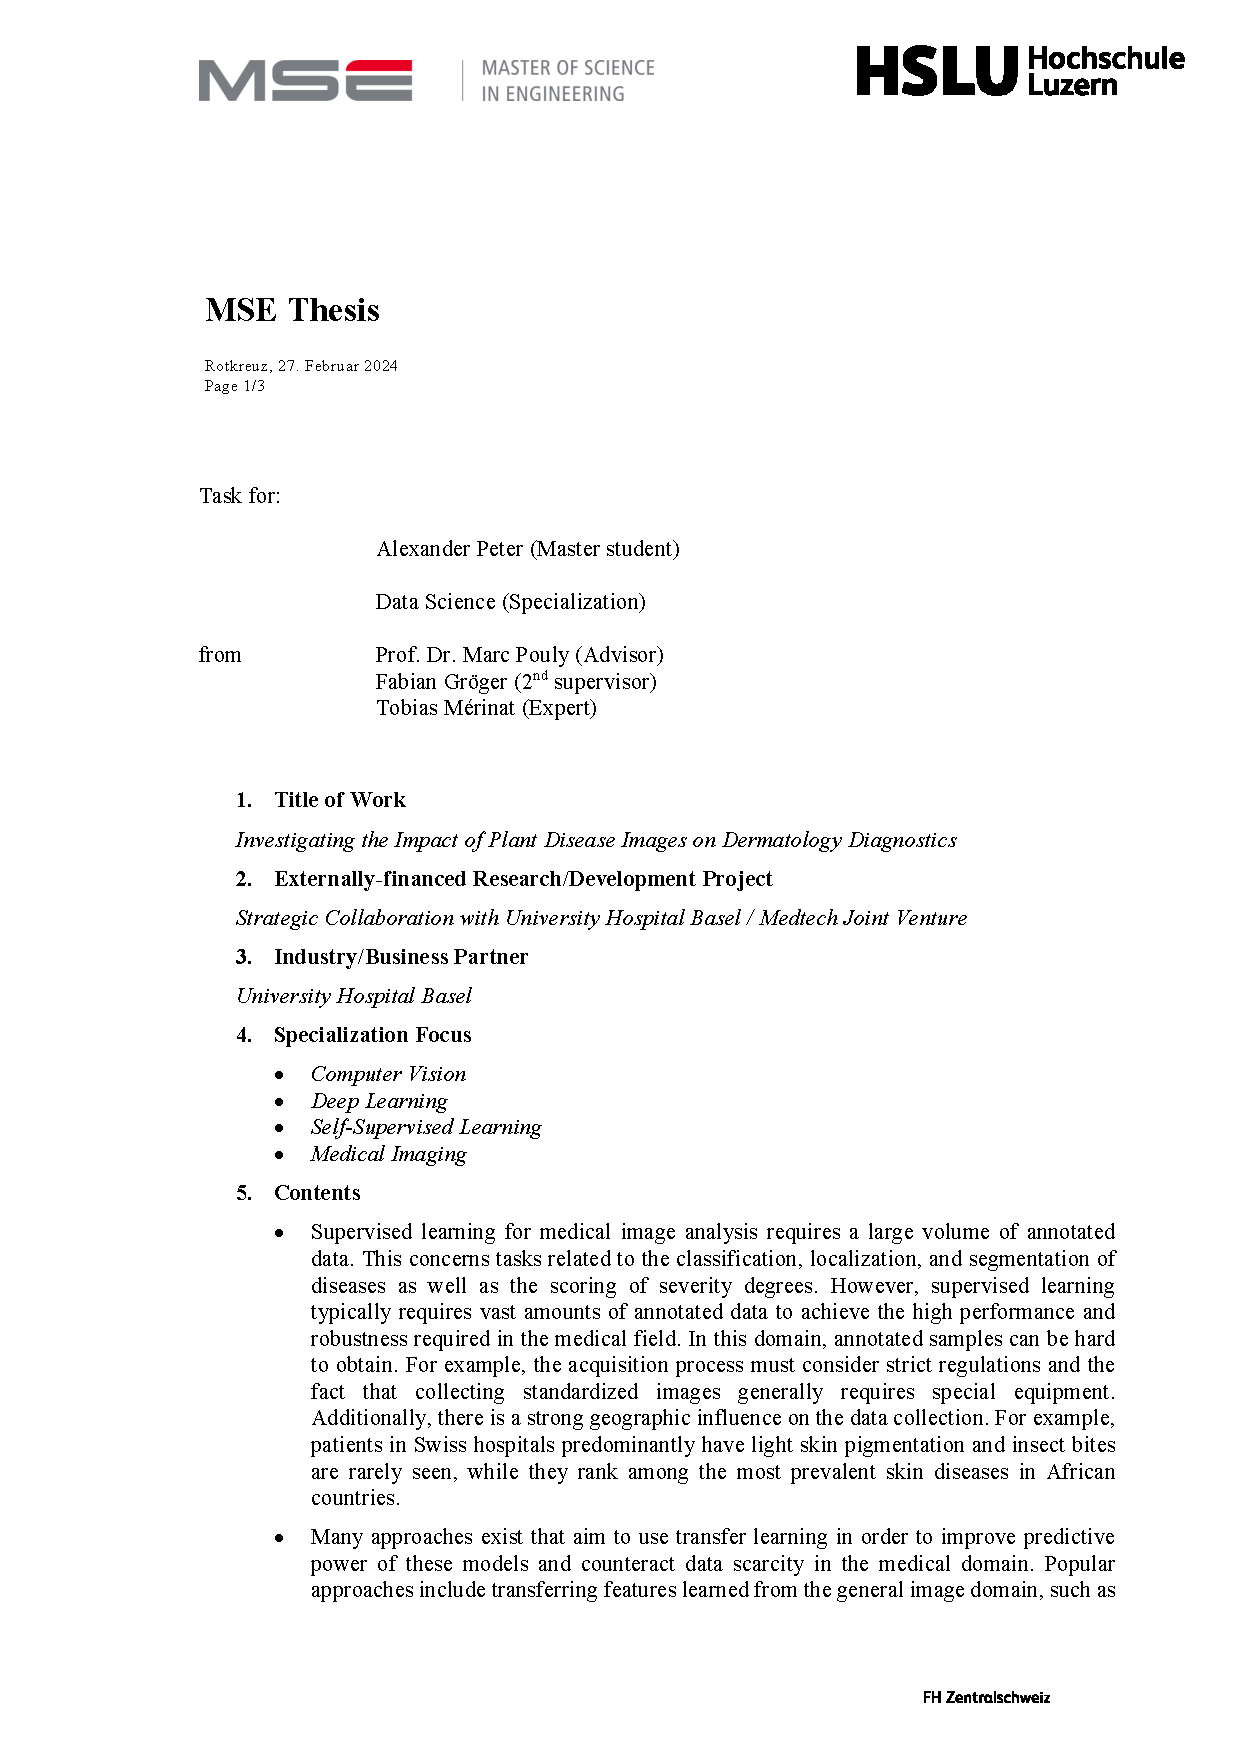
\includepdf[pages=-,addtotoc={1, section, 1, Task description, task description}]{../documents/task_description.pdf}
%TODO change to final version

\label{appendix:task_description}

\section{Meeting notes}
\label{subsection:notes}
% textidote: ignore begin
\markdownInput{../documents/meeting_notes.md}
% textidote: ignore end

\newpage
\section{Dataset collection}
\label{appendix:datasets_tables}
%TODO consider subsection
The following Table \ref{tab:all_plant_datasets} shows all plant disease datasets which could be found publicly available. 

\begin{table}[H]
\centering
\caption{Public plant disease datasets \label{tab:all_plant_datasets}}
\begin{tabularx}{\textwidth}{|
 >{\hsize=.50\hsize}X |
 >{\hsize=.14\hsize\raggedleft}X |
 >{\hsize=.14\hsize\raggedleft}X |
 >{\hsize=.22\hsize}X |
}
\hline
\textbf{Name} & \textbf{\#Images} & \textbf{\#Classes} & \textbf{Download} \\ \hline
PlantVillage (PVD) & 54'303 & 38 & \href{https://github.com/spMohanty/PlantVillage-Dataset}{\color{blue}{\underline{Github}}}\footnotemark{} \\ \hline
Cassava Leaf Disease Classification & 21'398 & 5 & \href{https://www.kaggle.com/competitions/cassava-leaf-disease-classification}{\color{blue}{\underline{Kaggle}}}\footnotemark{} \\ \hline
PlantDataset & 5'106 & 20 & \href{https://www.kaggle.com/datasets/duggudurgesh/plantdataset}{\color{blue}{\underline{Kaggle}}}\footnotemark{} \\ \hline
PlantDoc & 2'598 & 28 & \href{https://github.com/pratikkayal/PlantDoc-Dataset}{\color{blue}{\underline{Github}}}\footnotemark{} \\ \hline
Medicinal plantdataset & 8'206 & 16 & \href{https://www.kaggle.com/datasets/samundersingh/plantdataset}{\color{blue}{\underline{Kaggle}}}\footnotemark{} \\ \hline
Leaf Images & 4'502 & 2 & \href{https://data.mendeley.com/datasets/hb74ynkjcn/1}{\color{blue}{\underline{Mendeley Data}}}\footnotemark{} \\ \hline
Rice leaf disease dataset & 120 & 3 & \href{https://archive.ics.uci.edu/dataset/486/rice+leaf+diseases}{\color{blue}{\underline{UC Irvine}}}\footnotemark{} \\ \hline
Plant-Pathology-2020 & 3'651 & 38 & \href{https://www.kaggle.com/c/plant-pathology-2020-fgvc7/data}{\color{blue}{\underline{Kaggle}}}\footnotemark{} \\ \hline
Plant Pathology 2021 & 18'600 & 13 & \href{https://www.kaggle.com/competitions/plant-pathology-2021-fgvc8/data}{\color{blue}{\underline{Kaggle}}}\footnotemark{} \\ \hline
PlantCLEF & \~4'000'000  & \~80'000 & \href{https://www.aicrowd.com/challenges/lifeclef-2022-23-plant}{\color{blue}{\underline{AIcrowd}}}\footnotemark{} \\ \hline
Cotton Disease Dataset & 2'310  & 4 & \href{https://www.kaggle.com/datasets/janmejaybhoi/cotton-disease-dataset}{\color{blue}{\underline{Kaggle}}}\footnotemark{} \\ \hline
Cotton Leaf Disease & 1'786  & 4 & \href{https://www.kaggle.com/datasets/raaavan/cottonleafinfection}{\color{blue}{\underline{Kaggle}}}\footnotemark{} \\ \hline
Crop Pest and Disease Detection \newline (CCMT) & 24'881  & 22 & \href{https://data.mendeley.com/datasets/bwh3zbpkpv/1}{\color{blue}{\underline{Mendeley Data}}}\footnotemark{} \\ \hline
Maize with disease dataset & 18'222  & 2 & \href{https://osf.io/p67rz/}{\color{blue}{\underline{OSF}}}\footnotemark{} \\ \hline
DARMA & 231'414  & 1'000 & \href{https://drive.google.com/drive/folders/13bOuB7U15CgYMm1vrd0jgtOXFwMlHqXf}{\color{blue}{\underline{Google Drive}}}\footnotemark{} \\ \hline
Leaf disease segmentation dataset & 588  & 0 & \href{https://www.kaggle.com/datasets/fakhrealam9537/leaf-disease-segmentation-dataset}{\color{blue}{\underline{Kaggle}}}\footnotemark{} \\ \hline
CVPPP, LSC & 532  & 0 & \href{https://github.com/lxfhfut/Self-Supervised-Leaf-Segmentation}{\color{blue}{\underline{Github}}}\footnotemark{} \\ \hline
New Plant Diseases Dataset & 87'000  & 38 & \href{https://www.kaggle.com/datasets/vipoooool/new-plant-diseases-dataset/data}{\color{blue}{\underline{Kaggle}}}\footnotemark{} \\ \hline
Plant disease diagnosis dataset (PDDD) & 421'133  & 120 & \href{https://plantpad.samlab.cn/image\_down.html}{\color{blue}{\underline{PlantPAD}}}\footnotemark{} \\ \hline

\end{tabularx}
\end{table}

\addtocounter{footnote}{-19}
\stepcounter{footnote}\footnotetext{https://github.com/spMohanty/PlantVillage-Dataset}
\stepcounter{footnote}\footnotetext{https://www.kaggle.com/competitions/cassava-leaf-disease-classification}
\stepcounter{footnote}\footnotetext{https://www.kaggle.com/datasets/duggudurgesh/plantdataset}
\stepcounter{footnote}\footnotetext{https://github.com/pratikkayal/PlantDoc-Dataset}
\stepcounter{footnote}\footnotetext{https://www.kaggle.com/datasets/samundersingh/plantdataset}
\stepcounter{footnote}\footnotetext{https://data.mendeley.com/datasets/hb74ynkjcn/1}
\stepcounter{footnote}\footnotetext{https://archive.ics.uci.edu/dataset/486/rice+leaf+diseases}
\stepcounter{footnote}\footnotetext{https://www.kaggle.com/c/plant-pathology-2020-fgvc7/data}
\stepcounter{footnote}\footnotetext{https://www.kaggle.com/competitions/plant-pathology-2021-fgvc8/data}
\stepcounter{footnote}\footnotetext{https://www.aicrowd.com/challenges/lifeclef-2022-23-plant}
\stepcounter{footnote}\footnotetext{https://www.kaggle.com/datasets/janmejaybhoi/cotton-disease-dataset}
\stepcounter{footnote}\footnotetext{https://www.kaggle.com/datasets/raaavan/cottonleafinfection}
\stepcounter{footnote}\footnotetext{https://data.mendeley.com/datasets/bwh3zbpkpv/1}
\stepcounter{footnote}\footnotetext{https://osf.io/p67rz/}
\stepcounter{footnote}\footnotetext{https://drive.google.com/drive/folders/13bOuB7U15CgYMm1vrd0jgtOXFwMlHqXf}
\stepcounter{footnote}\footnotetext{https://www.kaggle.com/datasets/fakhrealam9537/leaf-disease-segmentation-dataset}
\stepcounter{footnote}\footnotetext{https://github.com/lxfhfut/Self-Supervised-Leaf-Segmentation}
\stepcounter{footnote}\footnotetext{https://www.kaggle.com/datasets/vipoooool/new-plant-diseases-dataset/data}
\stepcounter{footnote}\footnotetext{https://plantpad.samlab.cn/image\_down.html}